% !TEX root =../tfmETSI.tex
\chapter{Methodology}\label{chp:methodology}

\section{Overview}
\label{sec:meth-overview}

The chapter sets up the building blocks the rest of this work rests on: the contrastive vision-language paradigm under study (CLIP, §\ref{sec:meth-clip}), the encoders we plug into it (§\ref{sec:meth-image}, §\ref{sec:meth-text}), the training and external-evaluation datasets (§\ref{sec:meth-dataset}, §\ref{sec:meth-external-datasets}), the preprocessing and baseline configuration (§\ref{sec:meth-pre}, §\ref{sec:meth-baseline}), and the evaluation protocol that all experiments share (§\ref{sec:meth-eval}). The chapter ends with the compute and reproducibility setup (§\ref{sec:meth-compute}). Two reference baselines (PLIP zero-shot and a non-CLIP plain image classifier) run alongside the main experiment matrix; their configurations are described inline in the Results chapter where each is evaluated (§\ref{sec:results-plip-zeroshot}, §\ref{sec:results-foundational-vs-plain}).

The structure is intended to be read linearly --- background first, then the baseline configuration, then the experiments. Every experiment in the chapters that follow uses a single-variable-change design: each variant changes exactly one component of the baseline (image encoder, text encoder, input preprocessing, classifier head, or prompt format) and holds everything else identical, so that any observed delta on external evaluation traces back to that single change. The full experiment matrix --- which variant changes which axis --- is given in Table~\ref{tab:experiment-matrix} of Chapter~\ref{chp:results}.

Before going further, it is worth being clear about what this work does not attempt. We do not work with patient-level groupings (LC25000 is not patient-grouped), we do not run human-expert or clinical evaluation, and we do not include a controlled head-to-head against other histopathology foundation models (CONCH~\cite{lu2024conch}, BiomedCLIP~\cite{zhang2023biomedclip}, MUSK~\cite{xiang2025musk}). All three are listed as future work in Chapter~\ref{chp:conclusion}.


\section{Histopathology Digital Imaging}
\label{sec:meth-histo}

\subsection{Background}

Histopathology is the microscopic study of tissue removed from a patient to diagnose disease --- most commonly cancer. A biopsy or surgical specimen is fixed, embedded in paraffin, sliced into thin sections (typically 4--5\,µm), stained, and mounted on a glass slide for a pathologist to examine under a microscope. The pathologist's report is the gold-standard diagnosis that drives treatment decisions in oncology and many other specialties. Automating any meaningful part of this workflow --- triaging slides, flagging regions of interest, suggesting a diagnosis --- is one of the highest-impact targets for medical AI, both because pathologist time is a scarce resource and because the visual patterns involved are well-defined enough to be machine-learnable.

The stain used almost universally is hematoxylin and eosin (H\&E): hematoxylin colours cell nuclei a dark blue/purple, eosin colours cytoplasm and extracellular matrix pink. Slides are digitised by a Whole-Slide Imaging (WSI) scanner into a multi-gigapixel image (Figure~\ref{fig:wsi-multimag}), which is typically tiled into smaller patches (commonly $224 \times 224$ or $512 \times 512$ pixels at $20\times$ or $40\times$ magnification) for downstream learning, since current image encoders cannot process whole slides directly. Figure~\ref{fig:nct-crc-classes} shows the tissue-type variation a model has to discriminate between within a single dataset.

\begin{figure}[H]
    \centering
    \includegraphics[width=0.95\textwidth]{../results/plots/methodology/external/wsi_he_multimag_wikimedia.png}
    \caption{An H\&E-stained whole-slide image of breast tumour tissue at three magnification levels ($4\times$, $20\times$, $40\times$) over a $2.2$~cm$^2$ area. The slide-level view shows tissue architecture; higher magnifications reveal cellular detail used by pathologists for diagnosis. Image by KajsaMollersen, 2022; reproduced under CC-BY-SA 4.0.}
    \label{fig:wsi-multimag}
\end{figure}

\begin{figure}[H]
    \centering
    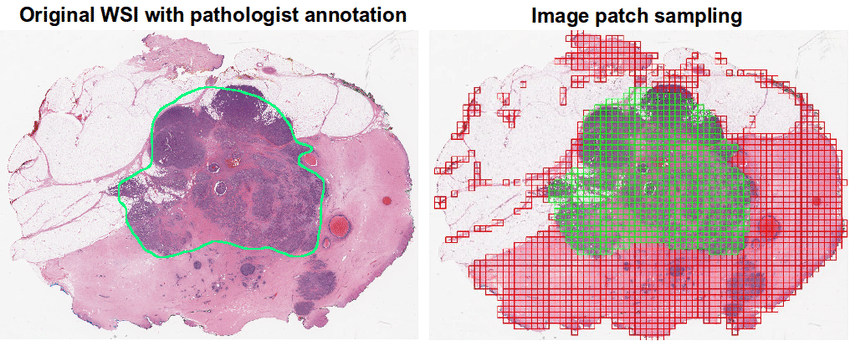
\includegraphics[width=0.85\textwidth]{../results/plots/methodology/external/wsi_patching_cruzroa2014.png}
    \caption{Patch-sampling on a whole-slide image. Left: original WSI with pathologist annotation (green outline) marking the cancer region. Right: the same WSI tiled into patches for downstream learning, with patch tiles intersecting the annotation marked in green and the rest in red. Reproduced from Cruz-Roa et al.~\cite{cruzroa2014idc}.}
    \label{fig:wsi-patching}
\end{figure}

\begin{figure}[H]
    \centering
    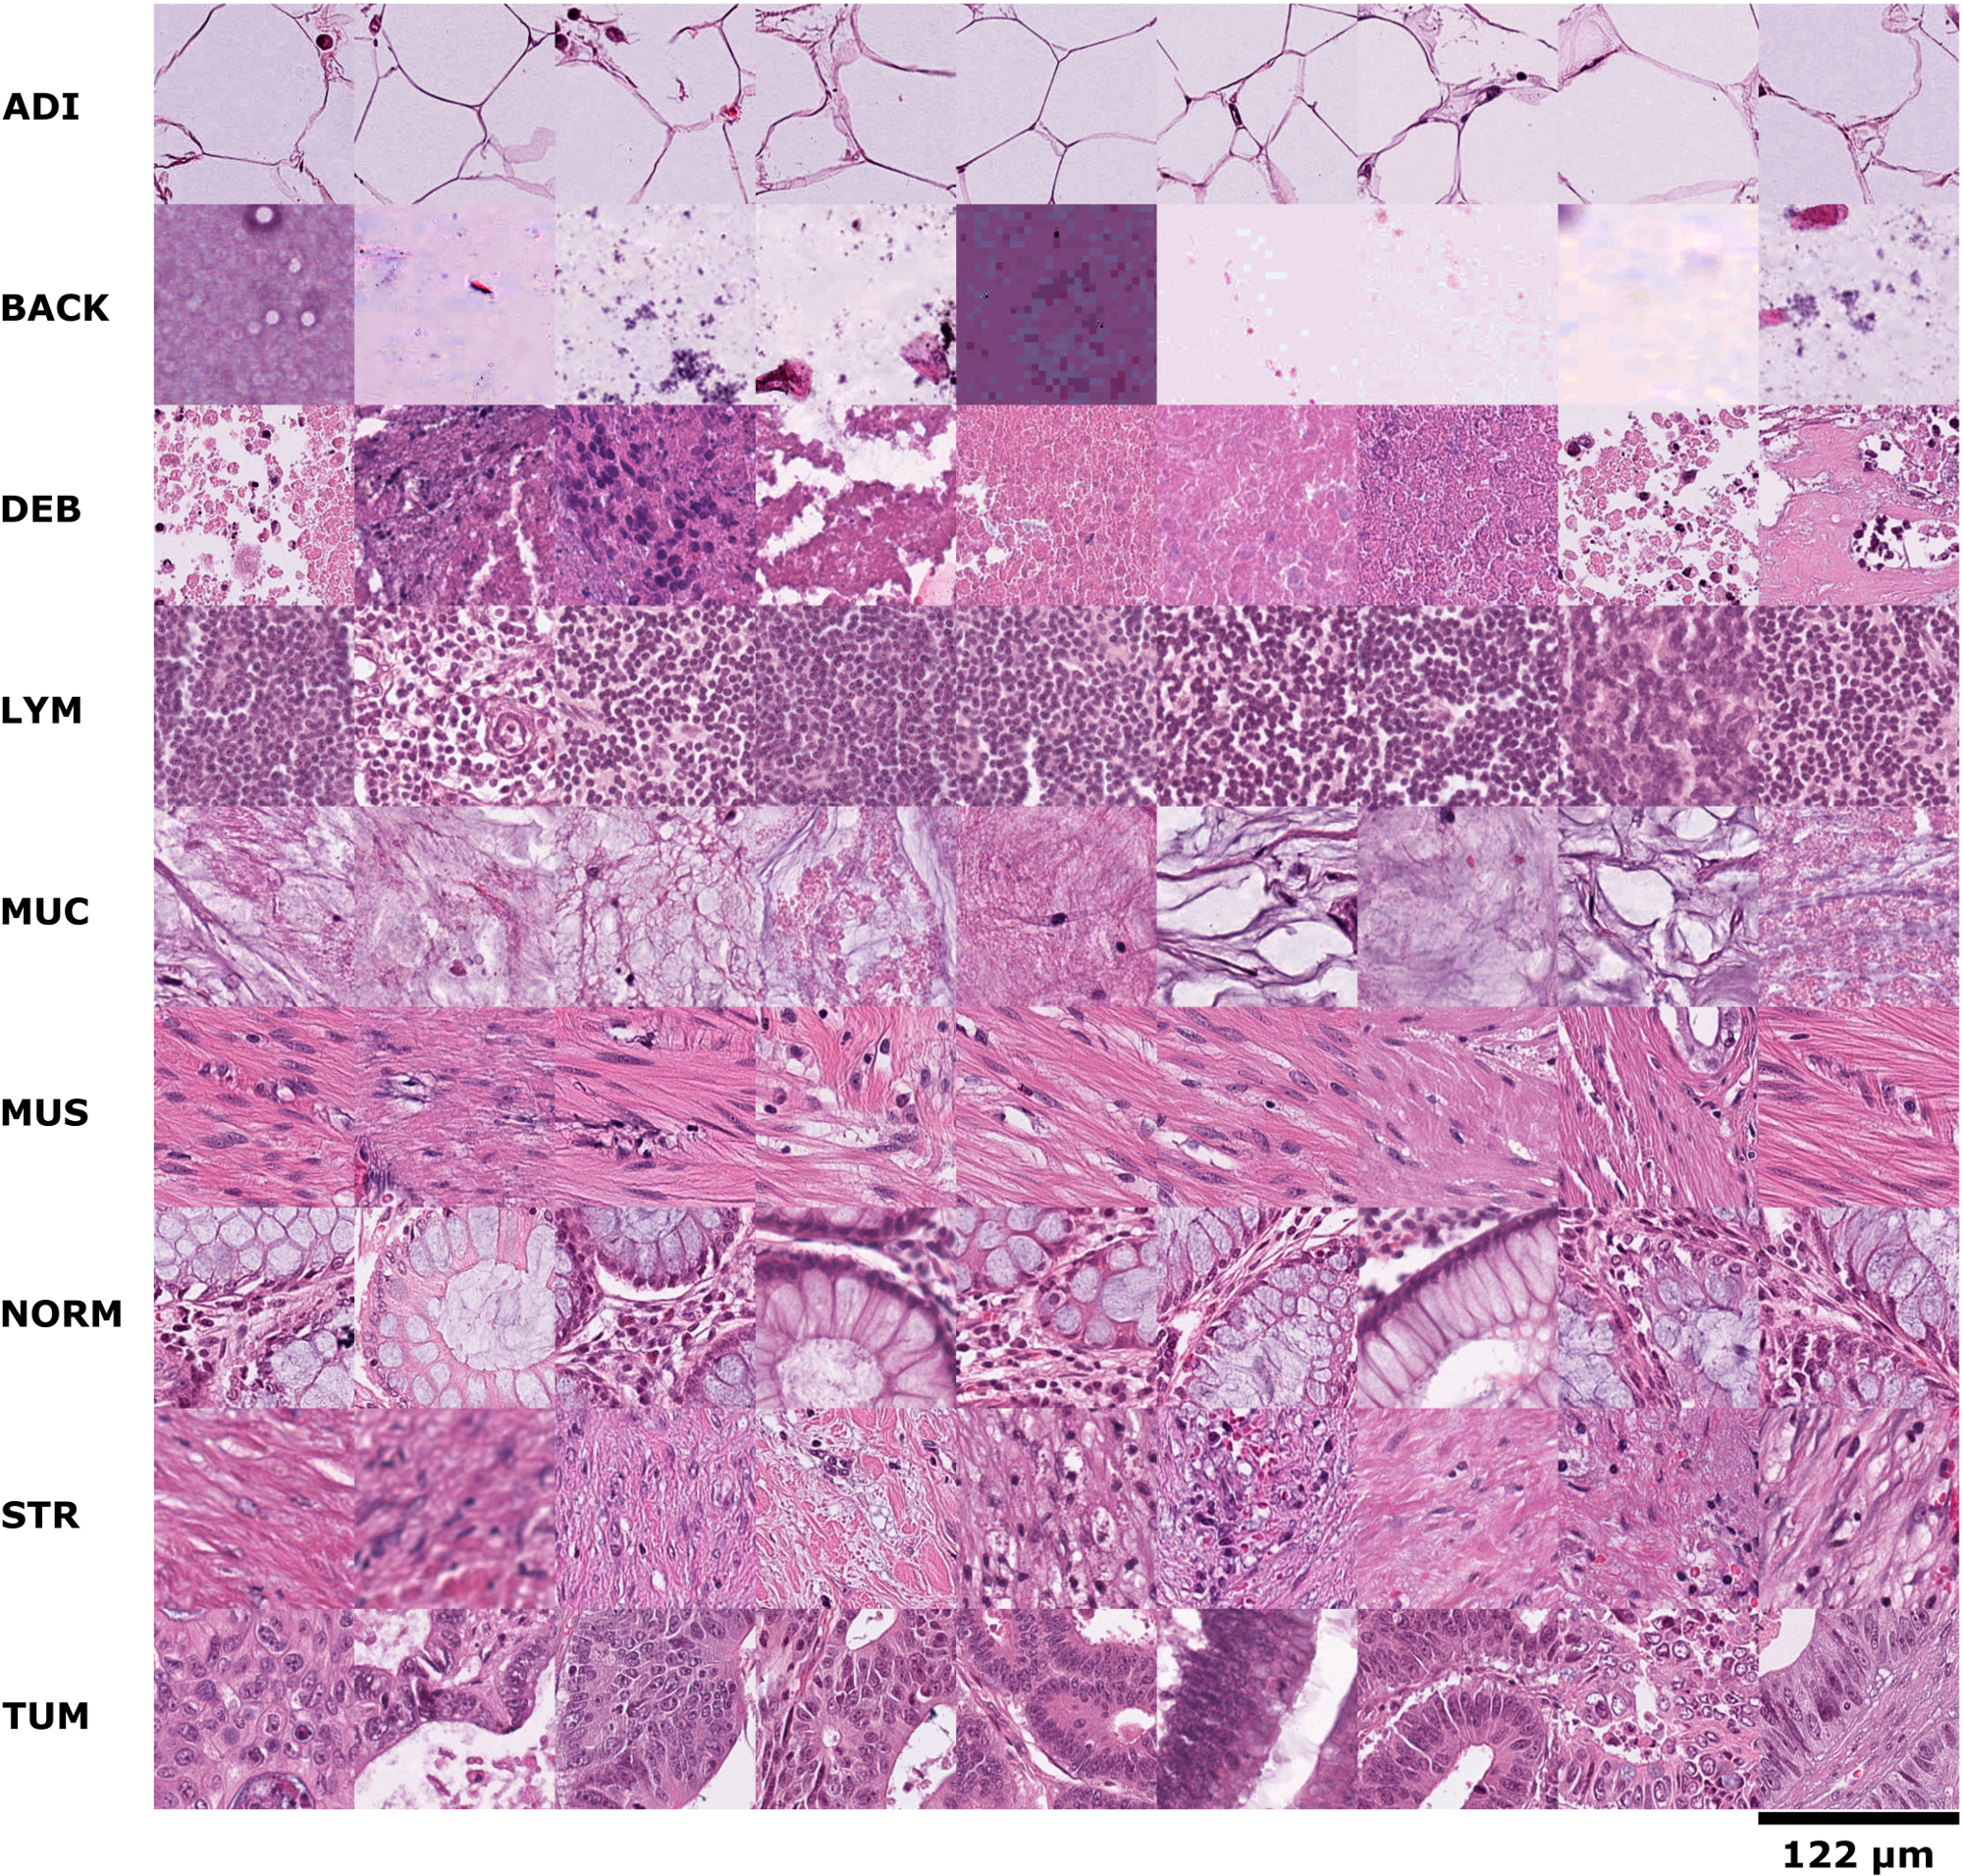
\includegraphics[width=0.85\textwidth]{../results/plots/methodology/external/nct_crc_classes_kather2019.png}
    \caption{Example H\&E patches from each of the nine tissue classes in the NCT-CRC-HE-100K dataset, illustrating the visual variation a histopathology classifier has to discriminate between within a single colorectal-cancer corpus. Figure~1 of Kather et al.~\cite{kather2019nct}, reproduced under the CC-BY 4.0 licence.}
    \label{fig:nct-crc-classes}
\end{figure}

\FloatBarrier

Several things make this domain hard for general-purpose vision-language models. Clinical archives rarely come with per-image natural-language captions of the kind that train CLIP at scale; pathology image--text corpora are small (PLIP's OpenPath has $\sim 208$k pairs, vs CLIP's $400$M for natural images) and noisier in their text. Several public histopathology datasets ship with subtle artifacts --- white-pixel skew, scanner-specific JPEG signatures, augmentation-pair leakage --- that can drive in-distribution performance without any meaningful tissue signal, motivating careful external evaluation. And finally, the visual signature of an H\&E slide depends heavily on the lab and scanner that produced it; that is the topic of the next subsection.

\subsection{Stain normalization in histopathology images}
\label{sec:meth-stain}

H\&E staining is not a deterministic procedure. The hematoxylin and eosin formulations, staining times, scanner colour profiles, and even individual technician handling all introduce variation in the resulting colour palette. Across institutions the variation is large and visible to the eye --- two slides of the same tissue type can look stylistically very different. Within a single institution it is smaller but still present, varying with technician shift, batch of reagents, and scanner calibration. This becomes a problem for any downstream classifier: a model trained on one institution's slides can latch onto that institution's specific stain signature rather than the underlying tissue pattern, then fail on a differently-stained slide of the same disease at evaluation time. Stain normalisation is the family of techniques that tries to remove the confounder by mapping every input into a common reference stain palette before downstream encoding.

Three normalisation methods are commonly cited: Macenko (stain-vector decomposition via SVD on the optical-density-transformed image)~\cite{macenko2009stain}, Reinhard (Lab-space colour-statistics transfer)~\cite{reinhard2001color}, and Vahadane (sparse non-negative matrix factorisation)~\cite{vahadane2016structure}. Figure~\ref{fig:stain-illustration} shows the same LC25000 patch under raw stain and each of the three normalisations --- the colour palette shifts visibly between methods, even though the underlying tissue content is identical. Macenko is the only method we advance to full external evaluation in this work. Reinhard and Vahadane were explored in an early pass but did not move forward: Vahadane's non-negative matrix factorisation solver fails to converge on a non-trivial fraction of LC25000 patches (see §\ref{sec:results-stain}, Figure~\ref{fig:stain-before-after}, for the full multi-class breakdown), and Reinhard is a Lab-space colour-statistics transfer rather than a true stain-decomposition method --- useful as a visual reference but not equivalent to Macenko's stain-vector approach.

Macenko's procedure operates in \textbf{optical-density (OD) space}. An RGB pixel intensity $I \in [0, 255]^3$ is first mapped to OD space by
\begin{equation}
\mathrm{OD} = -\log_{10}\!\left(\frac{I + 1}{I_0}\right), \qquad I_0 = 255,
\end{equation}
where the $+1$ avoids the singularity on pure-black pixels. In OD space, the two stains act as additive components, so each pixel decomposes as
\begin{equation}
\mathrm{OD} = S \cdot C,
\end{equation}
with $S \in \mathbb{R}^{3 \times 2}$ the stain-vector matrix (one 3-D colour vector per stain) and $C \in \mathbb{R}^{2}$ the per-stain concentration. Macenko estimates $S$ from the image by taking the SVD of the OD-space pixel cloud and choosing the two extreme directions in the top-2 singular-vector plane; the concentrations $C$ then follow by pseudo-inversion, $C = S^{+}\, \mathrm{OD}$. To normalise to a reference image with stain matrix $S_\mathrm{ref}$, the concentrations are preserved and re-projected through the reference stains:
\begin{equation}
\mathrm{OD}' = S_\mathrm{ref} \cdot C, \qquad I' = I_0 \cdot 10^{-\mathrm{OD}'}.
\end{equation}
Concretely, the procedure first \emph{learns} what colours the hematoxylin and eosin stains take in the input image, decomposes each pixel into those two components, and then re-renders the pixel using the colours those same stains take in the reference image.

\begin{figure}[H]
    \centering
    \begin{minipage}[t]{0.23\textwidth}
        \centering
        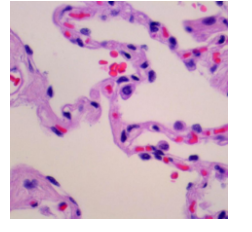
\includegraphics[width=\textwidth]{../results/plots/stain_single_raw.png}
        \par\vspace{2pt}\footnotesize (a) Raw.
    \end{minipage}\hfill
    \begin{minipage}[t]{0.23\textwidth}
        \centering
        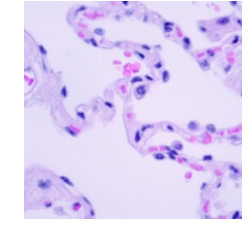
\includegraphics[width=\textwidth]{../results/plots/stain_single_macenko.png}
        \par\vspace{2pt}\footnotesize (b) Macenko.
    \end{minipage}\hfill
    \begin{minipage}[t]{0.23\textwidth}
        \centering
        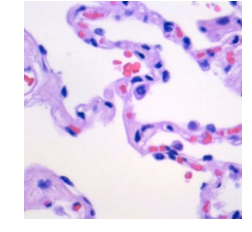
\includegraphics[width=\textwidth]{../results/plots/stain_single_reinhard.png}
        \par\vspace{2pt}\footnotesize (c) Reinhard.
    \end{minipage}\hfill
    \begin{minipage}[t]{0.23\textwidth}
        \centering
        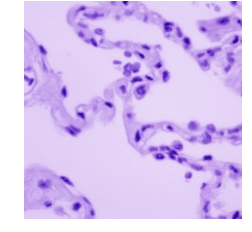
\includegraphics[width=\textwidth]{../results/plots/stain_single_vahadane.png}
        \par\vspace{2pt}\footnotesize (d) Vahadane.
    \end{minipage}
    \caption{Stain normalization comparison on a single LC25000 benign-lung patch. (a) Raw input, (b) Macenko-normalized, (c) Reinhard-normalized, (d) Vahadane-normalized. Each method produces a different colour palette from the same underlying tissue content. The full multi-class comparison, including the Vahadane convergence failure on some patches, is in §\ref{sec:results-stain}.}
    \label{fig:stain-illustration}
\end{figure}

\FloatBarrier

The reference patch is the first \texttt{NORM} tile from NCT-CRC-HE-7K, referred to as ``NCT-NORM'' throughout. Training applies Macenko(NCT-NORM) to every LC25000 patch before the encoder, which lands the training distribution near NCT-CRC's release stain space. At inference, the same Macenko(NCT-NORM) transform is applied to Chaoyang and LungHist700 (both arrive in their native stain palette), but NCT-CRC is fed raw: because NCT-CRC is already Macenko-normalised by Kather et al.~\cite{kather2019nct} before release, applying a second Macenko pass at inference would re-introduce a double-Macenko artefact that zeroed out performance in an earlier version of this experiment. The data-dependent direction this setup produces on external evaluation is the subject of §\ref{sec:results-stain}.


\section{Contrastive Vision-Language Learning (CLIP)}
\label{sec:meth-clip}

\subsection{Why CLIP?}

CLIP~\cite{radford2021clip} (Contrastive Language--Image Pretraining, Radford et al., 2021) is the contrastive vision-language paradigm under study in this work. Originally trained on $\sim 400$M image--text pairs scraped from the web, it learns to associate images with their natural-language descriptions in a shared embedding space and has become one of the most widely-used vision-language foundation models. The reason to centre the project on CLIP rather than on, say, a CNN with a softmax head is that CLIP's training signal --- aligning images with natural-language descriptions in a shared embedding space --- gives the model capabilities a closed-set classifier does not have. Three are directly relevant to histopathology classification:

\begin{itemize}
    \item \textbf{Open-vocabulary classification.} A new class can be introduced at inference time simply by writing a prompt for it; no retraining or label remapping is required. This is the property that lets CLIP be applied zero-shot to datasets it was never trained on.
    \item \textbf{Semantic similarity as the output.} CLIP returns a cosine-similarity score between an image and any text query --- not just a class label --- which makes retrieval and prompt-tuning natural downstream tasks.
    \item \textbf{Prompt engineering as a sensitivity lever.} Because classification depends on how each class is described in natural language, the prompt format itself becomes a tunable knob; we test this directly in §\ref{sec:results-text-encoder}.
\end{itemize}

A practical consequence is that CLIP is the \emph{object} of study in this work rather than the classifier per se. Every variant is evaluated via classification F1, but the broader question is what kind of representations CLIP produces under histopathology supervision, and what changes when individual components of the pipeline are swapped.

\subsection{Architecture and training signal}

The CLIP architecture is a dual-encoder (Figure~\ref{fig:clip-paradigm}): an image encoder and a text encoder, trained jointly so that matched image--text pairs land close together in a shared $d$-dimensional embedding space. Throughout this work we use $d = 256$, the dimensionality of the trained projection head's output. At inference, a sample is classified by encoding the image and each candidate class prompt, then taking the argmax of the cosine similarity between the image embedding and the class-prompt embeddings.

\noindent\textbf{InfoNCE loss.} For a batch of $N$ matched image--text pairs $\{(I_i, T_i)\}_{i=1}^{N}$, the model embeds each side into the shared $d$-dimensional space and produces two L2-normalised batches of embeddings, $\{\mathbf{v}_i\}$ and $\{\mathbf{t}_i\}$. Define the scaled cosine similarity between image $i$ and prompt $j$ as
\begin{equation}
s_{ij} \;=\; \frac{\mathbf{v}_i \cdot \mathbf{t}_j}{\tau},
\label{eq:scaled-cosine}
\end{equation}
where $\tau$ is the learnable temperature introduced below. For each image $i$ the image-to-text contrastive loss treats the matched prompt $i$ as the positive and the other $N{-}1$ prompts in the same batch as negatives; the row-wise softmax cross-entropy then reads
\begin{equation}
\mathcal{L}_{I \to T} \;=\; -\frac{1}{N} \sum_{i=1}^{N} \log \frac{\exp(s_{ii})}{\sum_{j=1}^{N} \exp(s_{ij})}.
\label{eq:infonce-i2t}
\end{equation}
The symmetric InfoNCE loss~\cite{oord2018cpc,radford2021clip} averages this with the analogous column-wise text-to-image loss $\mathcal{L}_{T \to I}$ (in which each prompt is matched against its image positive and the $N{-}1$ batch images as negatives):
\begin{equation}
\mathcal{L}_{\text{InfoNCE}} \;=\; \tfrac{1}{2} \left( \mathcal{L}_{I \to T} + \mathcal{L}_{T \to I} \right).
\label{eq:infonce-sym}
\end{equation}
Geometrically, minimising $\mathcal{L}_{\text{InfoNCE}}$ pulls matched (image, prompt) pairs together in cosine-similarity space and pushes the $N{-}1$ batch-internal mismatches apart.

\noindent\textbf{Learnable temperature.} The scalar $\tau$ in equation~\eqref{eq:scaled-cosine} controls the sharpness of the softmax in equation~\eqref{eq:infonce-i2t}: a smaller $\tau$ peaks the distribution and pushes the model toward sharply confident positives, while a larger $\tau$ smooths it. Following CLIP~\cite{radford2021clip} we store $\log(1/\tau)$ as the trainable variable (which guarantees $\tau > 0$ throughout training without an explicit constraint) and initialise it to $\log(1/0.07) \approx 2.66$, the CLIP-paper default. Gradient descent moves it freely during training. Empirically $\log(1/\tau)$ drifts upward (i.e.\ $\tau$ shrinks) as the embedding space stabilises, reflecting the model's preference for sharper positives as the contrastive task becomes easier; the converged value is reported alongside the loss curves in Chapter~\ref{chp:results}.

\noindent\textbf{Caveats.} The InfoNCE objective above assumes the $N{-}1$ in-batch negatives are \emph{genuine} mismatches. With our 5-class LC25000 supervision and batch size $N{=}32$ (Table~\ref{tab:baseline-hyperparameters}), the expected number of true mismatches per image is $0.8 \times (N{-}1) \approx 24.8$ but the expected number of \emph{false negatives} (other batch entries sharing the image's class, and therefore its prompt) is $\sim 6$. The loss therefore penalises some semantically-correct alignments. We do not mitigate this in the present study --- it is documented as a limitation in Chapter~\ref{chp:conclusion}.

Figure~\ref{fig:clip-paradigm} reproduces the canonical CLIP paradigm as introduced by Radford et al.~\cite{radford2021clip}: contrastive image--text pretraining (panel 1) builds a shared embedding space; class prompts then become the zero-shot classifier (panels 2--3). Figure~\ref{fig:clip-architecture} is the specific instantiation of that paradigm used in this work --- short histopathology class prompts, $256$-d projection heads on top of frozen foundation-model encoders, and a single fixed prompt strategy used at both training and evaluation time.

\begin{figure}[ht]
    \centering
    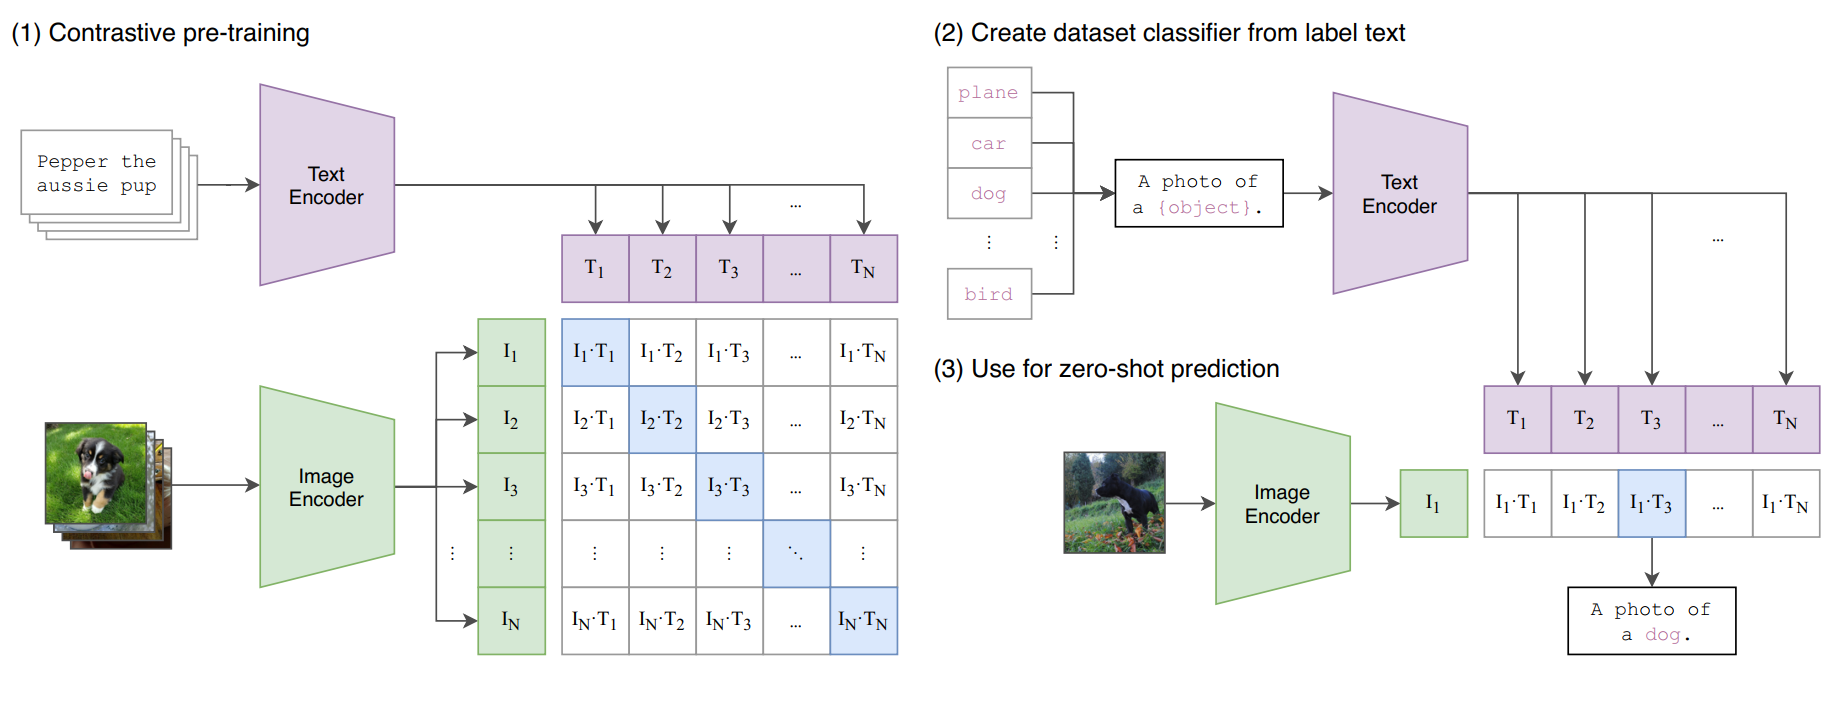
\includegraphics[width=0.95\textwidth]{../results/plots/methodology/clip_paradigm_radford2021.png}
    \caption{The CLIP paradigm as introduced by Radford et al., 2021 (Figure 1 of the original paper, reproduced for illustration). \textbf{(1) Contrastive pre-training}: two encoders project a batch of image--text pairs into a shared embedding space; the in-batch cosine-similarity matrix is supervised so the diagonal pairs (matched) score higher than off-diagonals (mismatched). \textbf{(2) Build a dataset-specific classifier from label text}: any new task is cast as text by encoding class-name prompts through the same text encoder. \textbf{(3) Zero-shot prediction}: an unseen image is classified by cosine-similarity argmax against the class prompts --- no task-specific training needed.}
    \label{fig:clip-paradigm}
\end{figure}

\begin{figure}[ht]
    \centering
    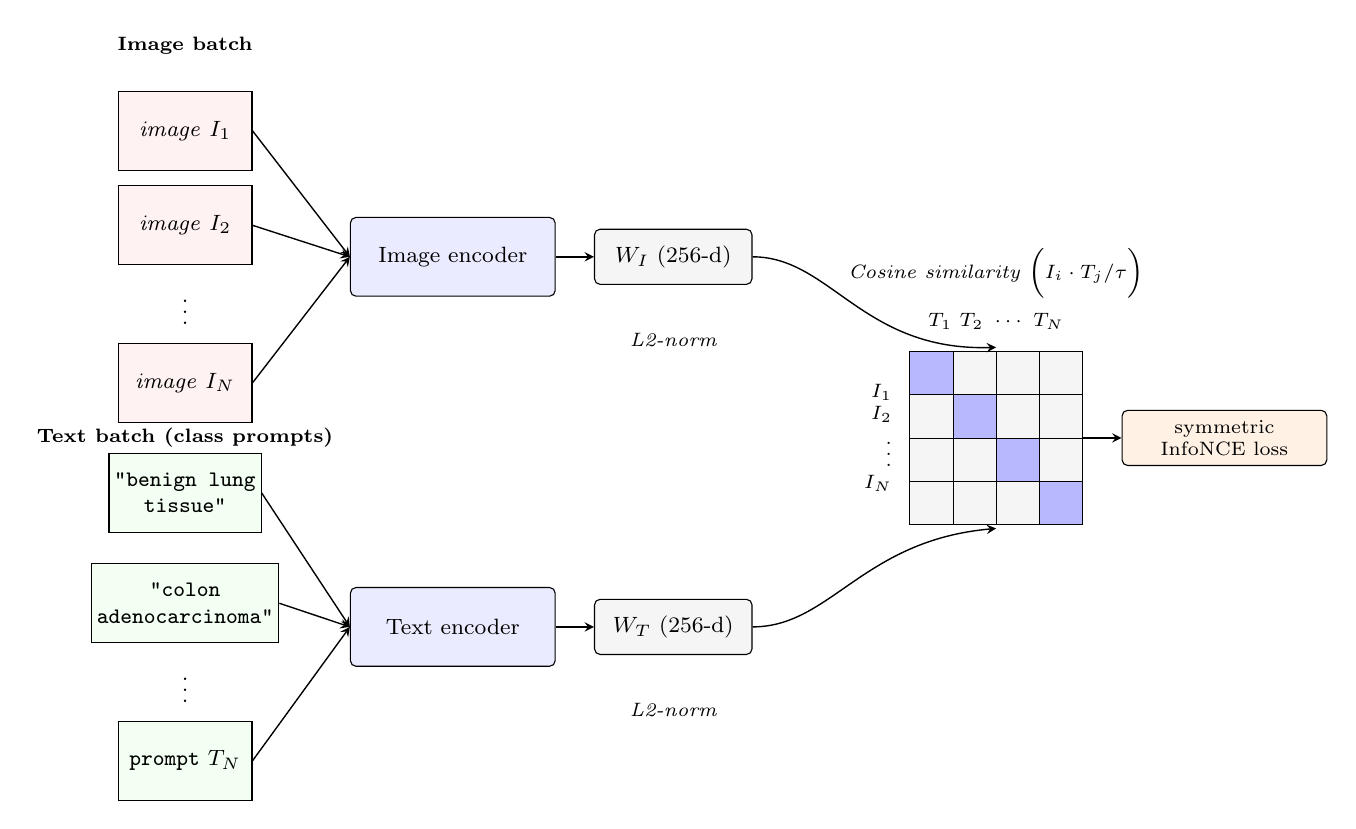
\begin{tikzpicture}[
        font=\footnotesize,
        x=1cm, y=1cm,
        encoder/.style ={draw, rounded corners=2pt, minimum width=2.6cm, minimum height=1.0cm,
                         fill=blue!8, line width=0.4pt},
        proj/.style    ={draw, rounded corners=2pt, minimum width=2.0cm, minimum height=0.7cm,
                         fill=gray!8, line width=0.4pt},
        sample/.style  ={draw, minimum width=1.7cm, minimum height=1.0cm, line width=0.4pt,
                         align=center, inner sep=2pt},
        emb/.style     ={draw, circle, minimum size=0.45cm, inner sep=0pt, line width=0.3pt},
        arr/.style     ={->, >=stealth, line width=0.5pt},
        >=stealth,
    ]
    %% Left -- inputs
    \node[sample, fill=red!5]  (img1) at (0,  1.6) {\textit{image} $I_1$};
    \node[sample, fill=red!5]  (img2) at (0,  0.4) {\textit{image} $I_2$};
    \node                       at (0, -0.6) {$\vdots$};
    \node[sample, fill=red!5]  (imgN) at (0, -1.6) {\textit{image} $I_N$};

    \node[sample, fill=green!5] (txt1) at (0, -3.0) {\texttt{"benign lung}\\\texttt{tissue"}};
    \node[sample, fill=green!5] (txt2) at (0, -4.4) {\texttt{"colon}\\\texttt{adenocarcinoma"}};
    \node                        at (0, -5.4) {$\vdots$};
    \node[sample, fill=green!5] (txtN) at (0, -6.4) {\texttt{prompt}~$T_N$};

    %% Encoders
    \node[encoder] (imenc) at (3.4,  0.0) {Image encoder};
    \node[encoder] (txenc) at (3.4, -4.7) {Text encoder};

    %% Projections
    \node[proj] (improj) at (6.2,  0.0) {$W_I$ (256-d)};
    \node[proj] (txproj) at (6.2, -4.7) {$W_T$ (256-d)};

    %% L2 / temperature
    \node[align=center, font=\scriptsize\itshape] at (6.2,  -1.05) {L2-norm};
    \node[align=center, font=\scriptsize\itshape] at (6.2,  -5.75) {L2-norm};

    %% Arrows: inputs -> encoder (fan-in to encoder's western edge)
    \foreach \src in {img1, img2, imgN}
        \draw[arr] (\src.east) -- (imenc.west);
    \foreach \src in {txt1, txt2, txtN}
        \draw[arr] (\src.east) -- (txenc.west);

    %% Encoders -> projections
    \draw[arr] (imenc) -- (improj);
    \draw[arr] (txenc) -- (txproj);

    %% Cosine similarity matrix
    \def\mx{9.2}      % left edge of matrix
    \def\my{-3.4}     % bottom edge of matrix
    \def\cs{0.55}     % cell size
    \pgfmathsetmacro{\mtop}{\my + 4*\cs}
    \pgfmathsetmacro{\mright}{\mx + 4*\cs}
    \foreach \i in {0,1,2,3} {
        \foreach \j in {0,1,2,3} {
            \pgfmathsetmacro{\cx}{\mx + \j*\cs}
            \pgfmathsetmacro{\cy}{\my + (3-\i)*\cs}
            \ifnum\i=\j
                \draw[fill=blue!28, line width=0.2pt] (\cx,\cy) rectangle ++(\cs,\cs);
            \else
                \draw[fill=gray!8,  line width=0.2pt] (\cx,\cy) rectangle ++(\cs,\cs);
            \fi
        }
    }
    %% Matrix labels
    \node[anchor=south, font=\scriptsize] at (\mx + 2*\cs, \mtop + 0.15) {$T_1\ T_2\ \cdots\ T_N$};
    \node[anchor=east,  font=\scriptsize, align=right]
        at (\mx - 0.10, \my + 2*\cs) {$I_1$\\$I_2$\\$\vdots$\\$I_N$};
    \node[anchor=south, font=\scriptsize\itshape] at (\mx + 2*\cs, \mtop + 0.55)
        {Cosine similarity $\bigl(I_i \cdot T_j / \tau\bigr)$};

    %% Projection -> matrix arrows
    \draw[arr] (improj.east) .. controls (8.2, 0) and (8.6, -1.2) .. (\mx + 2*\cs, \mtop + 0.05);
    \draw[arr] (txproj.east) .. controls (8.2, -4.7) and (8.6, -3.6) .. (\mx + 2*\cs, \my - 0.05);

    %% InfoNCE loss callout
    \node[draw, rounded corners=2pt, fill=orange!10, line width=0.4pt,
          minimum width=2.6cm, minimum height=0.7cm, align=center, font=\scriptsize]
          (loss) at (\mright + 1.8, \my + 2*\cs) {symmetric\\InfoNCE loss};
    \draw[arr] (\mright, \my + 2*\cs) -- (loss.west);

    %% Section labels
    \node[font=\scriptsize\bfseries, anchor=south] at (0,  2.45) {Image batch};
    \node[font=\scriptsize\bfseries, anchor=south] at (0, -2.55) {Text batch (class prompts)};

    \end{tikzpicture}
    \caption{CLIP dual-encoder architecture used in this project. Two independent encoders project a batch of $N$ image--text pairs into a shared $d$-dimensional embedding space (here $d = 256$, the projection head's output). After L2-normalisation and a learnable temperature $\tau$, the $N \times N$ cosine-similarity matrix between every image and every prompt is the input to the symmetric InfoNCE loss. The diagonal (blue) entries are the positive pairs; off-diagonal entries are negatives within the batch.}
    \label{fig:clip-architecture}
\end{figure}

\subsection{PLIP: a histopathology-pretrained CLIP-style model}
\label{sec:meth-plip-model}

PLIP~\cite{huang2023plip} (Huang et al., 2023) is a CLIP-style model pretrained on histopathology image--text pairs. Its training corpus is OpenPath, $\sim 208$k image--text pairs scraped from Twitter conversations among pathologists (using hashtags like \texttt{\#GIPath}, \texttt{\#PathTwitter}, etc.), supplemented with a filtered subset of LAION; the architecture is a CLIP ViT-B/32 vision encoder paired with a CLIP-style text encoder, both trained contrastively starting from CLIP's natural-image initialisation. Figure~\ref{fig:plip-openpath} illustrates the data pipeline: pathologist tweets become image--caption pairs that feed the contrastive training matrix, and over many training steps the image and matching-text embeddings get pulled together in the shared space.

\begin{figure}[H]
    \centering
    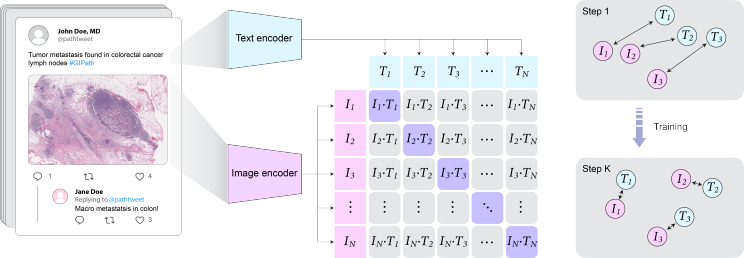
\includegraphics[width=0.95\textwidth]{../results/plots/methodology/external/plip_openpath_pipeline.png}
    \caption{The PLIP data pipeline and contrastive training. Left: a pathologist's Twitter post with an H\&E patch and a clinical description becomes an (image, text) training pair. Middle: PLIP's image and text encoders produce embeddings that are arranged into an $N \times N$ cosine-similarity matrix; the contrastive loss pulls the diagonal (matched) entries up and the off-diagonal entries down. Right: over many training steps, matched image--text pairs converge in the shared embedding space. Adapted from Huang et al.~\cite{huang2023plip}.}
    \label{fig:plip-openpath}
\end{figure}

\FloatBarrier

We use PLIP in two distinct ways. As a \emph{zero-shot reference baseline} (§\ref{sec:results-plip-zeroshot}), the full PLIP model --- image and text encoders both frozen --- is used off-the-shelf for cosine-similarity classification on all four datasets (LC25000 plus the three external evaluation sets). As a \emph{pretrained image encoder} in the image-encoder comparison (§\ref{sec:meth-image-vit}), only PLIP's ViT-B/32 vision encoder is used, paired with our LC25000-trained projection head and a separate BERT text encoder. The two roles isolate different questions: the first tests what pathology pretraining gives on its own; the second tests what pathology pretraining gives on top of LC25000 supervision.


\section{Image Encoders}
\label{sec:meth-image}

The image encoder is the component swapped in the central image-encoder comparison of this work (§\ref{sec:results-image-encoder}). Three encoders are compared: ResNet50 (§\ref{sec:meth-image-resnet}, the baseline's CNN, supervised on ImageNet); PLIP's ViT-B/32 (§\ref{sec:meth-image-vit}, the histopathology-contrastive ViT covered in §\ref{sec:meth-plip-model}); and DINOv2 ViT-B/14 (§\ref{sec:meth-image-dinov2}, general-domain self-supervised). The three were chosen to disentangle the three axes that change when ResNet50 is swapped for PLIP: the architecture (CNN vs ViT), the pretraining objective (supervised vs self-supervised vs contrastive), and the pretraining domain (natural images vs histopathology). DINOv2 specifically isolates ``ViT + self-supervision'' from ``histopathology pretraining'', acting as the control in the comparison.

A note on the following subsections: ResNet50 and DINOv2 below describe full encoder-plus-pretraining units, but the ViT subsection covers only the architecture --- the encoder we actually plug are PLIP's ViT-B/32 (already described in §\ref{sec:meth-plip-model}) and DINOv2's ViT-B/14. The two ViTs also differ in patch size (/32 vs /14), giving them different feature granularity at the same input resolution; this becomes a methodological caveat in the §\ref{sec:results-image-encoder} discussion.

\subsection{ResNet50 (CNN, ImageNet supervised)}
\label{sec:meth-image-resnet}

ResNet50~\cite{he2016resnet} (He et al., 2016) is the convolutional baseline. It is a deep residual network with $\sim 23$M parameters; the architecture's hallmark is the addition of skip connections that let gradients bypass groups of convolutional layers, which made it the first deep model that trained reliably at $50+$ layers. The output we use is the $2048$-d global-average-pooled feature vector from the final convolutional block. We use the standard ImageNet-1K supervised pretraining checkpoint ($\sim 1.3$M natural images, 1000 classes); no histopathology data is involved.

The role of ResNet50 in this work is as the general-purpose image-encoder baseline. Plugging it in as the image encoder carries the implicit assumption that ImageNet-supervised features transfer broadly enough to be useful on histopathology --- the assumption the encoder-swap comparison in §\ref{sec:results-image-encoder} tests directly.

\subsection{Vision Transformer (ViT)}
\label{sec:meth-image-vit}

The Vision Transformer~\cite{dosovitskiy2021vit} (ViT; Dosovitskiy et al., 2020) is the transformer architecture for images. Instead of convolution, the input image is split into a grid of fixed-size patches; each patch is linearly embedded as a token, and the resulting sequence is fed through a stack of transformer encoder layers with self-attention. The architecture has no built-in spatial bias of the kind a CNN's filters provide --- it learns spatial relationships from data, which is a large part of why ViTs need substantial pretraining to work well.

The variant we care about is ViT-Base (``B''), which has 12 transformer layers and a hidden size of 768. The suffix in names like ViT-B/16, ViT-B/32, ViT-B/14 denotes the patch size: a smaller patch means more tokens (finer spatial granularity) at the same input resolution. At our standard $224 \times 224$ input, ViT-B/32 produces $49$ patch tokens while ViT-B/14 produces $256$.

The role of this subsection is descriptive rather than operational: the actual image encoder we plug into the comparison is PLIP's pretrained ViT-B/32, already described in §\ref{sec:meth-plip-model}. The patch-size difference between PLIP's B/32 and DINOv2's B/14 is the methodological caveat previewed in the section intro and discussed in §\ref{sec:results-image-encoder}.

\subsection{DINOv2 (self-supervised on general natural images)}
\label{sec:meth-image-dinov2}

DINOv2~\cite{oquab2024dinov2} (Oquab et al., 2024) is a self-supervised Vision Transformer and the strongest general-purpose visual SSL backbone available at the time of writing, positioned by its authors as a default frozen feature extractor across a wide range of downstream vision tasks --- classification, segmentation, depth estimation, retrieval --- without task-specific fine-tuning. It builds on the original DINO~\cite{caron2021dino} framework (Caron et al., 2021), which introduced self-distillation for vision transformers, and scales it substantially: a larger curated training corpus, larger backbones, and a number of training-stability improvements.

The training corpus is LVD-142M, $\sim 142$M curated general natural images assembled by Meta from a $1.2$B raw image pool via retrieval-based curation; there are no class labels, no captions, and no histopathology data. The training signal is self-distillation: the model is split into a student and a teacher network with the same ViT architecture, and the student is trained to match the teacher's output on different augmented crops of the same image (Figure~\ref{fig:dino-framework}). The teacher is updated as an exponential moving average of the student's weights, so all supervision comes from the consistency of representations across augmentations --- no external labels are involved. The augmentation strategy is \emph{multi-crop}: the student sees both global crops (large, full-context views) and local crops (small, zoomed-in views) of the same image, while the teacher sees only the global crops. Notably, DINOv2 is \emph{not} a contrastive method --- there are no in-batch negatives and no InfoNCE loss; the consistency objective alone provides the supervision signal.

\begin{figure}[H]
    \centering
    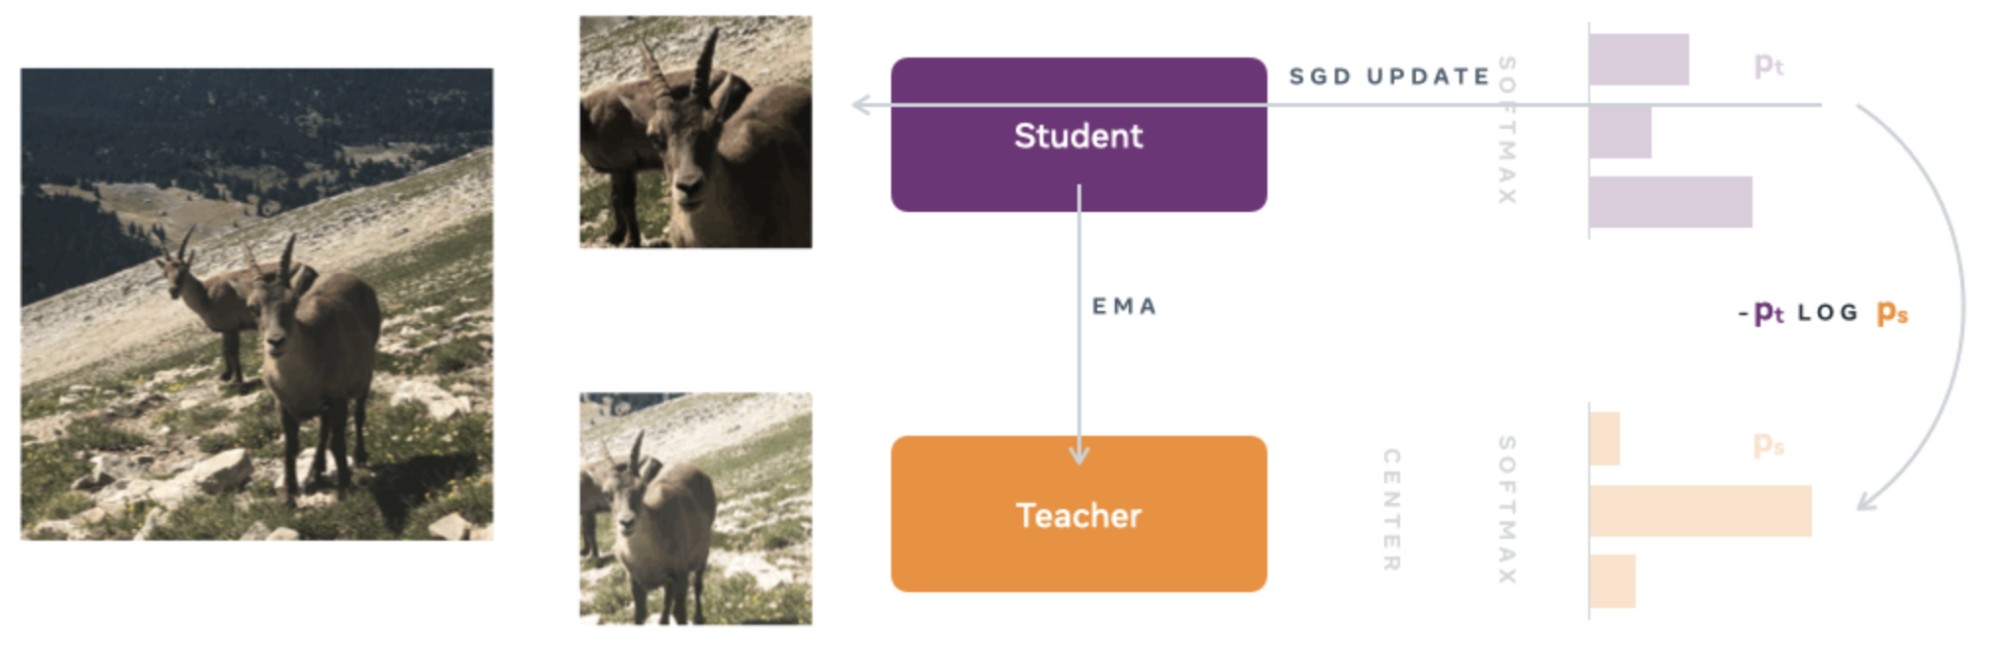
\includegraphics[width=0.85\textwidth]{../results/plots/methodology/external/dino_teacher_student.png}
    \caption{The DINO self-distillation framework used by DINOv2. Two augmented crops of the same image are fed through a student network and a teacher network; both produce softmax probability distributions $p_s$ and $p_t$. The student is trained via cross-entropy ($-p_t \log p_s$) to match the teacher's output and is updated by standard SGD; the teacher is updated as an exponential moving average (EMA) of the student's weights and is never directly trained. Adapted from Caron et al.~\cite{caron2021dino}.}
    \label{fig:dino-framework}
\end{figure}

\FloatBarrier

DINOv2 is released in four sizes (ViT-S/14, B/14, L/14, g/14, ranging from $\sim 22$M to $\sim 1.1$B parameters). We use ViT-B/14: the same Base architecture (12 layers, hidden 768) as PLIP's encoder, but with $14 \times 14$ patches rather than $32 \times 32$, giving the $256$ patch tokens noted above.

The role of DINOv2 in this work is as the control in the image-encoder comparison. It shares the architecture family (ViT) and the self-supervised paradigm with PLIP's vision encoder but never sees a histopathology image during pretraining. Plugging DINOv2 in as the image encoder therefore isolates ``ViT + general-domain self-supervision'' from ``histopathology pretraining specifically'': if DINOv2 closes the gap to PLIP, the win is largely architectural; if it does not, the win is specifically about histopathology pretraining.


\section{Text Encoders}
\label{sec:meth-text}

The text encoder is the second component swapped, in the text-encoder comparison of §\ref{sec:results-text-encoder}. Three encoders are compared, all from the BERT family~\cite{devlin2019bert} (Devlin et al., 2019), so the underlying architecture --- a 12-layer Transformer~\cite{vaswani2017attention} with 768-d hidden states and WordPiece tokenisation --- is the same across them; what differs is the corpus each encoder was pretrained on.

The baseline text encoder is \texttt{bert-base-uncased}, BERT trained on BookCorpus + English Wikipedia. The two biomedical variants are:

\begin{itemize}
    \item \textbf{BioBERT}~\cite{lee2020biobert} (Lee et al., 2020): a BERT-base checkpoint that starts from the BERT initialisation and is further pretrained on PubMed abstracts and PMC full-text articles, on top of the original BERT corpus.
    \item \textbf{PubMedBERT}~\cite{gu2021pubmedbert} (Gu et al., 2021): a BERT-base checkpoint pretrained \emph{from scratch} on PubMed abstracts and PMC, with a biomedical-vocabulary WordPiece tokeniser rather than the general-English one.
\end{itemize}

WordPiece tokenisation splits each input word into subword pieces drawn from a fixed vocabulary: rare or compound words decompose into multiple pieces (with a leading \texttt{\#\#} marking each continuation), while common words tokenise as a single piece. A special \texttt{[CLS]} token is prepended to every input and a \texttt{[SEP]} token closes it; the pooled embedding read out of the \texttt{[CLS]} position is what the projection head receives.

The vocabulary differs across the three encoders. BERT and BioBERT share the same general-English WordPiece vocabulary --- BioBERT inherits BERT's tokeniser and only continues pretraining on biomedical text. PubMedBERT trains a custom WordPiece vocabulary from scratch on PubMed and PMC text, so domain terms are far more likely to be single tokens. Table~\ref{tab:bert-tokenization} shows the resulting fragmentation for the baseline's composed prompt: BERT and BioBERT both split ``histopathology'' into four pieces and ``adenocarcinoma'' into four or five, while PubMedBERT keeps both as single tokens. This is a concrete reason a biomedical encoder could in principle help downstream classification --- the §\ref{sec:results-text-encoder} comparison tests whether the advantage translates into measurable F1 gains.

\begin{table}[H]
    \centering
    \small
    \begin{tabular}{|l|p{0.6\textwidth}|c|}
    \hline
    \textbf{Encoder} & \textbf{Tokens for ``A histopathology image of lung adenocarcinoma''} & \textbf{\#} \\ \hline
    BERT       & \texttt{[CLS] a his \#\#top \#\#ath \#\#ology image of lung aden \#\#oca \#\#rc \#\#ino \#\#ma [SEP]} & 15 \\ \hline
    BioBERT    & \texttt{[CLS] a his \#\#top \#\#ath \#\#ology image of lung ad \#\#eno \#\#car \#\#cin \#\#oma [SEP]} & 15 \\ \hline
    PubMedBERT & \texttt{[CLS] a histopathology image of lung adenocarcinoma [SEP]} & 8 \\ \hline
    \end{tabular}
    \caption{WordPiece tokenisation of the baseline composed prompt across the three text encoders. PubMedBERT's domain-trained vocabulary handles ``histopathology'' and ``adenocarcinoma'' as single tokens; BERT and BioBERT share BERT's general-English vocabulary, which fragments both terms into multiple wordpieces.}
    \label{tab:bert-tokenization}
\end{table}

All three encoders are dropped into the same baseline pipeline without other changes, isolating ``text-encoder pretraining'' as a single variable. The §\ref{sec:results-text-encoder} comparison crosses these three encoders with two prompt-format variants (bare class name vs ``A histopathology image of \{class\}.''), giving the 6-cell grid evaluated on NCT-CRC and extended to Chaoyang and LungHist700 for the best biomedical cell.


\section{Training Dataset: LC25000}
\label{sec:meth-dataset}

LC25000~\cite{borkowski2019lc25000} (Borkowski et al., 2019) is the only dataset used for training in this work. It contains five tissue classes spanning two organs --- benign lung tissue, lung adenocarcinoma, lung squamous cell carcinoma, benign colon tissue, and colon adenocarcinoma (Figure~\ref{fig:lc25000-samples}) --- with $5\,000$ patches per class for a total of $25\,000$ patches at $768 \times 768$ resolution. The patches are derived from $1\,250$ source images ($250$ per class) via geometric augmentation: each source is expanded into $20$ patches by random rotation and horizontal/vertical flipping; we do not add further augmentation on top. Table~\ref{tab:lc25000-splits} shows the stratified $80/10/10$ train/val/test split we use.

\textbf{Augmentation-pair leakage.} Because the $20$ augmented patches per source share image content, randomly splitting the $25\,000$ patches lets augmented copies of the same source image fall on both sides of the train/test split. We do not mitigate this in the runs reported here; it is flagged as a limitation in Chapter~\ref{chp:conclusion}. The leakage inflates in-distribution numbers --- every trained variant in this work saturates LC25000 at $\sim 0.99$ macro-F1 --- but does not affect the external-evaluation results that drive the chapter's conclusions, since no LC25000 source images appear in any external dataset.

The dataset has other known limits: it is a single-institution release, may contain stain artifacts, and lacks patient-level grouping or clinical validation. These are discussed in §\ref{sec:concl-limitations}.

\begin{figure}[H]
    \centering
    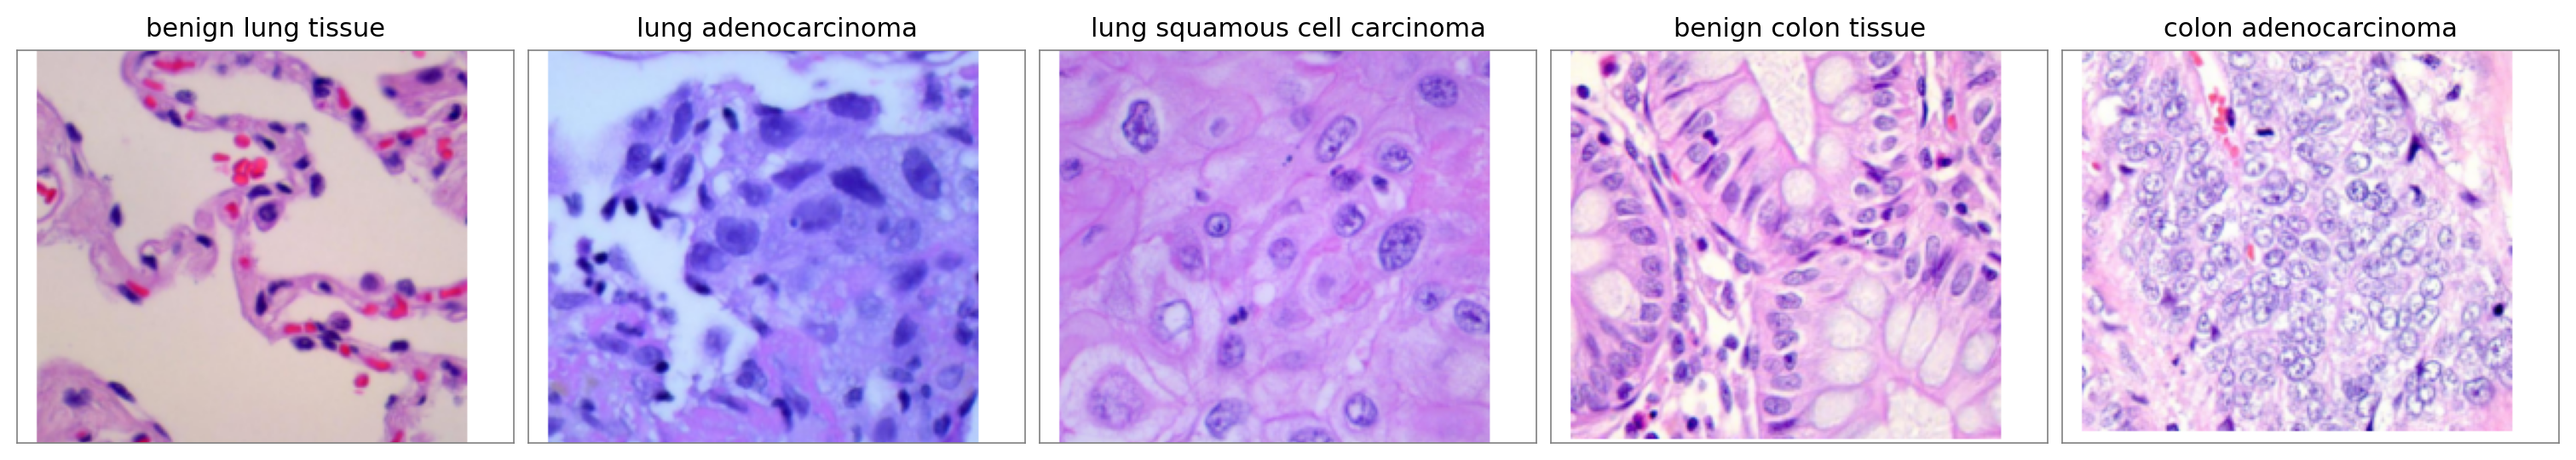
\includegraphics[width=0.95\textwidth]{../results/plots/methodology/lc25000_class_samples.png}
    \caption{Example image per class from LC25000. Left-to-right: benign lung tissue, lung adenocarcinoma, lung squamous cell carcinoma, benign colon tissue, colon adenocarcinoma. The two benign classes appear visually distinct from the cancer classes; within the cancers, lung adenocarcinoma vs lung squamous cell carcinoma is the hardest discrimination in our experiments (and a clinical confound).}
    \label{fig:lc25000-samples}
\end{figure}

\begin{table}[H]
    \centering
    \begin{tabular}{|l|c|c|c|c|}
    \hline
    \textbf{Class} & \textbf{Total} & \textbf{Train} & \textbf{Val} & \textbf{Test} \\ \hline
    benign lung tissue              & 5\,000 & 4\,000 & 500 & 500 \\ \hline
    lung adenocarcinoma             & 5\,000 & 4\,000 & 500 & 500 \\ \hline
    lung squamous cell carcinoma    & 5\,000 & 4\,000 & 500 & 500 \\ \hline
    benign colon tissue             & 5\,000 & 4\,000 & 500 & 500 \\ \hline
    colon adenocarcinoma            & 5\,000 & 4\,000 & 500 & 500 \\ \hline
    \textbf{Total}                  & 25\,000 & 20\,000 & 2\,500 & 2\,500 \\ \hline
    \end{tabular}
    \caption{LC25000 class counts and stratified split sizes.}
    \label{tab:lc25000-splits}
\end{table}

\FloatBarrier


\section{External Evaluation Datasets}
\label{sec:meth-external-datasets}

Each LC25000-trained variant is evaluated on three external datasets the model has never seen during training. The three are presented below in order of increasing shift severity relative to LC25000.

\subsection{NCT-CRC-HE-7K}

NCT-CRC-HE-7K~\cite{kather2019nct} (Kather et al., 2019; Zenodo record 1214456) is a colorectal-cancer patch dataset with $7\,180$ patches across 9 tissue classes. We restricted the evaluation to the (NORM $\leftrightarrow$ benign colon tissue) and (TUM $\leftrightarrow$ colon adenocarcinoma) classes that map to LC25000, giving $1\,974$ patches scored (741 NORM + 1\,233 TUM). The patches are $224 \times 224$ at $\sim 20\times$ magnification and arrive Macenko-normalised at release. NCT-CRC-HE-7K is the \textbf{close-shift colon} evaluation, stylistically similar to LC25000's colon side.

\subsection{Chaoyang}

Chaoyang~\cite{zhu2021chaoyang} (Zhu et al., 2022; preprint 2021) is a colorectal-cancer patch dataset from Beijing Chaoyang Hospital, $6\,160$ patches across 4 classes (normal, serrated, adenocarcinoma, adenoma). We restrict to normal ($\leftrightarrow$ benign colon, $n = 1\,816$) and adenocarcinoma ($\leftrightarrow$ colon adeno, $n = 2\,244$) for $4\,060$ patches scored. The patches are $512 \times 512$ at $20\times$, from a different hospital, scanner, and staining protocol than LC25000. The training split has documented label noise; the test split is labelled by consensus of three pathologists, and is the only split we use. Chaoyang is the \textbf{different-hospital colon} evaluation.

\subsection{LungHist700}

LungHist700~\cite{tabatabaei2024lunghist} (Tabatabaei et al., 2024, \emph{Scientific Data}) is a lung tissue dataset with $\sim 691$ high-resolution images at $20\times$ and $40\times$ magnifications, covering normal lung tissue plus adenocarcinoma and squamous-cell carcinoma at three differentiation grades each. We restrict to the $20\times$ subset for 3-class scoring: 359 images (85 normal, 146 adenocarcinoma, 128 squamous cell carcinoma). LungHist700 is the \textbf{different-source lung} evaluation, and the only multi-class external scoring in this work.


\section{Preprocessing and Input Pipeline}
\label{sec:meth-pre}

\subsection{Image preprocessing (per-backbone)}

Each image encoder expects pixel values in the distribution it was pretrained on, so the preprocessing we apply depends on which backbone we're using (Table~\ref{tab:image-preprocessing}). All inputs are resized to $224 \times 224$ with bilinear interpolation before they hit the encoder. We don't add any further augmentation on top: LC25000 already ships with rotation/flip augmentation at release, and the external evaluation sets are used as-is.

\begin{table}[H]
    \centering
    \small
    \begin{tabular}{|l|p{0.72\textwidth}|}
    \hline
    \textbf{Backbone} & \textbf{Preprocessing} \\ \hline
    ResNet50            & RGB / $255.0$ (i.e.\ $[0, 1]$ linear scaling) \\ \hline
    ViT-B/32 (PLIP)     & CLIP-standard mean/std normalisation: mean $=[0.481, 0.458, 0.408]$, std $=[0.269, 0.261, 0.276]$ \\ \hline
    ViT-B/14 (DINOv2)   & ImageNet mean/std normalisation: mean $=[0.485, 0.456, 0.406]$, std $=[0.229, 0.224, 0.225]$ \\ \hline
    \end{tabular}
    \caption{Per-backbone image preprocessing. Each backbone expects the input distribution it was pretrained on; mismatched preprocessing produces degraded features (see §\ref{sec:meth-preprocessing-bug}).}
    \label{tab:image-preprocessing}
\end{table}

\subsection{Text preprocessing}

All text encoders in this work use BERT-family WordPiece tokenisers (BERT, BioBERT, PubMedBERT, and PLIP's text encoder). We pad or truncate every input to a fixed sequence length of 24 tokens, which leaves comfortable headroom for every class-prompt format we test. The baseline's composed prompt template is \texttt{"A histopathology image of \{class\_name\}."}.

\subsection{LC25000-specific cleanup}

We apply two cleanup passes to LC25000 before training. First, we generate a canonical $80/10/10$ stratified train/val/test split with seed $42$ and check it into the repository as JSON, so every variant we train uses the exact same partition. Second, an MD5 pass over LC25000's files turns up $1\,280$ byte-identical duplicates, which we exclude via a dedupe-exclusion list (\texttt{src/data/lc25000\_dedupe\_exclusions.json}). One catch: the canonical split file pre-dates the dedupe pass, so the duplicates still cross the train/test boundary in the runs reported here. We flag this as a limitation in §\ref{sec:concl-limitations}.

\subsection{Methodological note on preprocessing}
\label{sec:meth-preprocessing-bug}

One bug worth recording surfaced mid-project. For a while, the pipeline was applying Caffe-style BGR mean-subtraction to a backbone that expected $[0, 1]$ RGB --- the mismatch came from two libraries shipping different ResNet50 checkpoints under the same name. The bug surfaced when a simple linear-probe diagnostic on the frozen features came back with a macro-F1 \emph{higher} than the trained CLIP ceiling, which should not happen. We fixed it by routing every image read through a centralised loader (\texttt{src/data/images.py}). The broader takeaway is methodological: linear-probing a frozen feature extractor against the trained model's ceiling is a cheap sanity check worth running early in any project.


\section{The Baseline}
\label{sec:meth-baseline}

The baseline pipeline is a frozen ResNet50 image encoder paired with a frozen BERT-base-uncased text encoder, with two small projection heads (\texttt{Dense(256, bias=False)} $\rightarrow$ \texttt{LayerNorm}) mapping each side into the shared $256$-d embedding space. Only the projection heads and the learnable temperature $\tau$ (initialised at $0.07$ following CLIP) are trained. The loss is symmetric InfoNCE, optimised with AdamW and gradient clipping; the same composed prompt template is used at training and at inference. All computation runs in float32. Table~\ref{tab:baseline-hyperparameters} gives the full hyperparameter list. Each variant in the experiment matrix changes exactly one row of this table; everything else is held constant.

\begin{table}[H]
    \centering
    \begin{tabular}{|l|l|}
    \hline
    \textbf{Hyperparameter} & \textbf{Value} \\ \hline
    Image encoder              & ResNet50 (ImageNet preset), frozen \\ \hline
    Text encoder               & BERT base uncased, frozen \\ \hline
    Projection head            & Dense(256, no bias) $\to$ LayerNorm \\ \hline
    Embedding dimension        & 256 \\ \hline
    Image size                 & $224 \times 224$ \\ \hline
    Text sequence length       & 24 WordPiece tokens \\ \hline
    Batch size                 & 32 \\ \hline
    Initial temperature        & $\tau = 0.07$ \\ \hline
    Loss                       & symmetric InfoNCE \\ \hline
    Optimizer                  & AdamW \\ \hline
    Learning rate              & $1 \times 10^{-3}$ \\ \hline
    Weight decay               & $1 \times 10^{-4}$ \\ \hline
    Gradient clipnorm          & 1.0 \\ \hline
    Max epochs                 & 30 \\ \hline
    EarlyStopping patience     & 5 \\ \hline
    ReduceLROnPlateau          & factor 0.5, patience 2, min $10^{-6}$ \\ \hline
    Numerical precision        & float32 \\ \hline
    Random seed                & 42 \\ \hline
    \end{tabular}
    \caption{Baseline hyperparameters. Each variant in the experiment matrix changes exactly one row.}
    \label{tab:baseline-hyperparameters}
\end{table}

\FloatBarrier


\section{Evaluation Protocol}
\label{sec:meth-eval}

\subsection{Metrics and visualizations}

We use two classification rules, depending on the variant. CLIP variants predict by taking the argmax of cosine similarity between the image embedding and the five LC25000 class-prompt embeddings; the plain classifier (§\ref{sec:results-foundational-vs-plain}) predicts by taking the argmax of the softmax over its \texttt{Dense(5)} output. All the metrics reported in the Results chapter follow from one of these two rules.

The global metrics reported throughout this work are:
\begin{itemize}
    \item \textbf{Accuracy} --- the fraction of samples whose predicted class matches the true class:
    $$\text{Accuracy} = \frac{1}{N} \sum_{i=1}^{N} \mathbb{1}[\hat{y}_i = y_i].$$
    \item \textbf{Balanced accuracy} --- the macro-average of per-class recall: equal weight to every class regardless of its support, so a single-class predictor on an imbalanced dataset cannot game the metric:
    $$\text{Balanced Accuracy} = \frac{1}{K} \sum_{k=1}^{K} R_k, \qquad R_k = \frac{\mathrm{TP}_k}{\mathrm{TP}_k + \mathrm{FN}_k}.$$
    \item \textbf{Macro-F1} --- the macro-average of per-class F1 (harmonic mean of precision and recall), again with equal weight per class. This is the headline metric throughout, chosen because external evaluations have imbalanced class supports and macro-F1 penalises class collapse symmetrically:
    $$\text{Macro-F1} = \frac{1}{K} \sum_{k=1}^{K} F1_k, \qquad F1_k = \frac{2 \, P_k R_k}{P_k + R_k}.$$
    \item \textbf{Weighted F1} --- per-class F1 weighted by class support; emphasises majority classes. Reported alongside macro-F1 for completeness:
    $$\text{Weighted F1} = \sum_{k=1}^{K} \frac{n_k}{N} \cdot F1_k.$$
\end{itemize}

We additionally report per-class precision, recall, F1, and support for every variant, along with confusion matrices (both raw counts and row-normalised by true class). For visualisations we produce a shared image-and-prompt UMAP on the training source (LC25000 test split), one fit per variant with points colour-coded by class; and a cross-distribution UMAP grid per external dataset where LC25000 image embeddings (circles, by class) are overlaid with external-dataset embeddings (triangles, by class) in a single shared UMAP fit per external dataset. All UMAPs use \texttt{umap-learn} with $n\_\text{neighbors}=15$, $\text{min\_dist}=0.1$, and cosine distance, fit on the L2-normalised projection-head output.

\subsection{External-dataset evaluation: restricted-argmax protocol}

External datasets cover only a subset of LC25000's classes --- NCT-CRC and Chaoyang are colon-only, LungHist700 is lung-only --- so an unrestricted argmax over all five LC25000 prompts would routinely predict the model's strongest out-of-organ class on these images and produce uninformative misclassifications. To avoid this, on external evaluation we restrict the argmax to the LC25000 classes that map to the external dataset's organ:

\begin{itemize}
    \item NCT-CRC and Chaoyang (colon datasets): argmax over \{benign colon tissue, colon adenocarcinoma\}.
    \item LungHist700 (lung dataset): argmax over \{benign lung tissue, lung adenocarcinoma, lung squamous cell carcinoma\}.
\end{itemize}

The full class-mapping rules per dataset are detailed in §\ref{sec:meth-external-datasets}. All external evaluation is pure inference: every variant reuses its LC25000-trained checkpoint with no fine-tuning on the external sets.

\subsection{Per-organ reporting}

Results in this work are reported per external dataset, never averaged across them. Averaging would hide the cross-organ regime change we see in Chapter~\ref{chp:results}: a single number across all external datasets would collapse the order-of-magnitude difference between the colon and lung sides into one misleading point. Reporting per-dataset is therefore an explicit choice driven by what the experiments showed, not the convenient default.


\section{Computational Setup and Reproducibility}
\label{sec:meth-compute}

All training and evaluation runs in this work were carried out on Google Colab (T4 GPU instances, occasionally L4 for the longer runs), with a local CPU/GPU fallback used for development and analysis. The main software stack is TensorFlow with KerasHub, which handles the CLIP-style training pipeline and every downstream evaluation. An auxiliary PyTorch + HuggingFace \texttt{transformers} stack is used only for image-encoder feature extraction when an encoder lacks a TensorFlow port (DINOv2, discussed below). Library versions are pinned in \texttt{requirements.txt} so the environment can be reproduced exactly.

Reproducibility is set up at three layers: a fixed random seed of $42$ across NumPy, TensorFlow, and PyTorch; \texttt{PYTHONHASHSEED} set explicitly; and \texttt{tf.config.experimental.enable\_op\_determinism()} called at the start of each run. Under these settings, repeat runs on the same hardware are bit-exact. Small numerical drift can appear across GPU types (T4 vs L4) due to floating-point ordering inside CUDA kernels, but it does not change the classification outcomes reported.

One practical caveat: DINOv2 has no TensorFlow port in our environment, so its image features are precomputed once in PyTorch and cached to disk as HDF5 files (one per dataset, keyed by image relative path). The TensorFlow training and evaluation pipelines then read from cache. This is mathematically equivalent to running the frozen backbone online --- the backbone is frozen, so every image always produces the same feature vector --- and it avoids the cost of running DINOv2 inference at every training step. The total cache footprint is $\sim 100$~MB across LC25000 and the three external datasets.
